%%%%%%%%%%%%%%%%%%%%%%%%%%%%%%%%%%%%%%%%%
% Wenneker Article
% LaTeX Template
% Version 2.0 (28/2/17)
%
% This template was downloaded from:
% http://www.LaTeXTemplates.com
%
% Authors:
% Vel (vel@LaTeXTemplates.com)
% Frits Wenneker
%
% License:
% CC BY-NC-SA 3.0 (http://creativecommons.org/licenses/by-nc-sa/3.0/)
%
%%%%%%%%%%%%%%%%%%%%%%%%%%%%%%%%%%%%%%%%%

%----------------------------------------------------------------------------------------
%	PACKAGES AND OTHER DOCUMENT CONFIGURATIONS
%----------------------------------------------------------------------------------------


%\documentclass[10pt, a4paper, twocolumn]{article}
\documentclass[10pt, a4paper]{article}% 10pt font size (11 and 12 also possible), A4 paper (letterpaper for US letter) and two column layout (remove for one column)

%%%%%%%%%%%%%%%%%%%%%%%%%%%%%%%%%%%%%%%%%
% Wenneker Article
% Structure Specification File
% Version 1.0 (28/2/17)
%
% This file originates from:
% http://www.LaTeXTemplates.com
%
% Authors:
% Frits Wenneker
% Vel (vel@LaTeXTemplates.com)
%
% License:
% CC BY-NC-SA 3.0 (http://creativecommons.org/licenses/by-nc-sa/3.0/)
%
%%%%%%%%%%%%%%%%%%%%%%%%%%%%%%%%%%%%%%%%%

%----------------------------------------------------------------------------------------
%	PACKAGES AND OTHER DOCUMENT CONFIGURATIONS
%----------------------------------------------------------------------------------------

\usepackage[spanish]{babel} % English language hyphenation

\usepackage{microtype} % Better typography

\usepackage{amsmath,amsfonts,amsthm} % Math packages for equations

%\usepackage[svgnames]{xcolor} % Enabling colors by their 'svgnames'

% \usepackage[hang, small, labelfont=bf, up, textfont=it]{caption} % Custom captions under/above tables and figures

\usepackage{booktabs} % Horizontal rules in tables

\usepackage{lastpage} % Used to determine the number of pages in the document (for "Page X of Total")

% \usepackage{graphicx} % Required for adding images

\usepackage{enumitem} % Required for customising lists
\setlist{noitemsep} % Remove spacing between bullet/numbered list elements

\usepackage{sectsty} % Enables custom section titles
\allsectionsfont{\usefont{OT1}{phv}{b}{n}} % Change the font of all section commands (Helvetica)

\usepackage{hyperref} % Required for hyperlinks
\hypersetup{hidelinks,colorlinks,breaklinks=true,urlcolor=Blue,citecolor=Green,linkcolor=DarkBlue,bookmarksopen=false,pdftitle={Title},pdfauthor={Author}}

\usepackage{lipsum} % Required to insert dummy text. To be removed otherwise
\usepackage{listings} % Para la parte de los keywords

%----------------------------------------------------------------------------------------
%	MARGINS AND SPACING
%----------------------------------------------------------------------------------------

% \usepackage{geometry} % Required for adjusting page dimensions

% \geometry{
% 	top=1cm, % Top margin
% 	bottom=1.5cm, % Bottom margin
% 	left=2cm, % Left margin
% 	right=2cm, % Right margin
% 	includehead, % Include space for a header
% 	includefoot, % Include space for a footer
% 	%showframe, % Uncomment to show how the type block is set on the page
% }

% \setlength{\columnsep}{7mm} % Column separation width

%----------------------------------------------------------------------------------------
%	FONTS
%----------------------------------------------------------------------------------------

\usepackage[T1]{fontenc} % Output font encoding for international characters
\usepackage[utf8]{inputenc} % Required for inputting international characters

\usepackage{XCharter} % Use the XCharter font

%----------------------------------------------------------------------------------------
%	HEADERS AND FOOTERS
%----------------------------------------------------------------------------------------

% \usepackage{fancyhdr} % Needed to define custom headers/footers
% \pagestyle{fancy} % Enables the custom headers/footers

% \renewcommand{\headrulewidth}{0.0pt} % No header rule
% \renewcommand{\footrulewidth}{0.4pt} % Thin footer rule

% \renewcommand{\sectionmark}[1]{\markboth{#1}{}} % Removes the section number from the header when \leftmark is used

%\nouppercase\leftmark % Add this to one of the lines below if you want a section title in the header/footer

% % Headers
% \lhead{} % Left header
% \chead{\textit{\thetitle}} % Center header - currently printing the article title
% \rhead{} % Right header

% % Footers
% \lfoot{} % Left footer
% \cfoot{} % Center footer
% \rfoot{\footnotesize Page \thepage\ of \pageref{LastPage}} % Right footer, "Page 1 of 2"

%\fancypagestyle{firstpage}{ % Page style for the first page with the title
% 	\fancyhf{}
% 	\renewcommand{\footrulewidth}{0pt} % Suppress footer rule
% }

%----------------------------------------------------------------------------------------
%	TITLE SECTION
%----------------------------------------------------------------------------------------

%\newcommand{\keywordname}{Keywords} % Defines the keywords heading name
\newcommand{\keywordname}{Keywords: \color{DarkBlue}} % Defines the keywords heading name

\newcommand{\authorstyle}[1]{{\large\usefont{OT1}{phv}{b}{n}\color{DarkRed}#1}} % Authors style (Helvetica)

\newcommand{\institution}[1]{{\footnotesize\usefont{OT1}{phv}{m}{sl}\color{Black}#1}} % Institutions style (Helvetica)

\usepackage{titling} % Allows custom title configuration

\newcommand{\HorRule}{\color{DarkGoldenrod}\rule{\linewidth}{1pt}} % Defines the gold horizontal rule around the title

\pretitle{
	\vspace{-55pt} % Move the entire title section up
	\HorRule\vspace{10pt} % Horizontal rule before the title
	\fontsize{24}{30}\usefont{OT1}{phv}{b}{n}\selectfont % Helvetica
	\color{DarkRed} % Text colour for the title and author(s)
}

\posttitle{\par\vskip 15pt} % Whitespace under the title

\preauthor{} % Anything that will appear before \author is printed

\postauthor{ % Anything that will appear after \author is printed
	\vspace{10pt} % Space before the rule
	\par\HorRule % Horizontal rule after the title
	\vspace{-45pt} % Space after the title section
}

%----------------------------------------------------------------------------------------
%	ABSTRACT
%----------------------------------------------------------------------------------------

\usepackage{lettrine} % Package to accentuate the first letter of the text (lettrine)
\usepackage{fix-cm}	% Fixes the height of the lettrine

\newcommand{\initial}[1]{ % Defines the command and style for the lettrine
	\lettrine[lines=1,findent=4pt,nindent=0pt]{% Lettrine takes up 3 lines, the text to the right of it is indented 4pt and further indenting of lines 2+ is stopped
		\color{DarkGoldenrod}% Lettrine colour
		{#1}% The letter
	}{}%
}

\usepackage{xstring} % Required for string manipulation

\newcommand{\lettrineabstract}[1]{
	\StrLeft{#1}{1}[\firstletter] % Capture the first letter of the abstract for the lettrine
	\initial{\firstletter}\textbf{\StrGobbleLeft{#1}{1}} % Print the abstract with the first letter as a lettrine and the rest in bold
}

%----------------------------------------------------------------------------------------
%	BIBLIOGRAPHY
%----------------------------------------------------------------------------------------

\usepackage[backend=bibtex,style=authoryear,natbib=true]{biblatex} % Use the bibtex backend with the authoryear citation style (which resembles APA)

\addbibresource{example.bib} % The filename of the bibliography

\usepackage[autostyle=true]{csquotes} % Required to generate language-dependent quotes in the bibliography
 % Specifies the document structure and loads requires packages
\usepackage[sc]{mathpazo} % Use the Palatino font
\usepackage[T1]{fontenc} % Use 8-bit encoding that has 256 glyphs
\linespread{1.05} % Line spacing - Palatino needs more space between lines
%\usepackage{microtype} % Slightly tweak font spacing for aesthetics

\usepackage[twoside,width=16cm,height=24cm,left=3cm]{geometry}
%\usepackage[hmarginratio=1:1,top=20mm,width=19cm,height=23cm,columnsep=15pt]{geometry} % Document margins
\usepackage{multicol} % Used for the two-column layout of the document
\usepackage[hang, small,labelfont=bf,up,textfont=it,up]{caption} % Custom captions under/above floats in tables or figures
\usepackage{booktabs} % Horizontal rules in tables
\usepackage{float} % Required for tables and figures in the multi-column environment - they need to be placed in specific locations with the [H] (e.g. \begin{table}[H])
\usepackage{hyperref} % For hyperlinks in the PDF

%----------- Agregados para el caso de ustedes -------------------------------
\usepackage[spanish]{babel}% idioma castellano
\usepackage[utf8]{inputenc}% esto es para poder poner los tildes directamente. Puede que cambie de versión a versión de sistema operativos (más información en http://www.aq.upm.es/Departamentos/Fisica/agmartin/webpublico/latex/FAQ-CervanTeX/FAQ-CervanTeX-6.html )
\usepackage{graphicx} % para insertar figuras
\usepackage{subfigure} % para insertar figuras dentro de figuras
\usepackage{times} % plataforma
\usepackage{amsmath} % --para ecuaciones y algunos símbolos 
% ---------------------- -----------------------------------------------------

\usepackage{lettrine} % The lettrine is the first enlarged letter at the beginning of the text
%\usepackage{paralist} % Used for the compactitem environment which makes bullet points with less space between them


\usepackage{abstract} % Allows abstract customization
\renewcommand{\abstractnamefont}{\normalfont\bfseries} % Set the "Abstract" text to bold
\renewcommand{\abstracttextfont}{\normalfont\itshape} % Set the abstract itself to small italic text
\addto\captionsspanish{ % Modifica algunos nombres cambiandolos por los definidos a continuacion
        \def\contentsname{\'Indice}%
        \def\bibname{Referencias}%
        \def\tablename{Tabla}%
        \def\abstractname{Resumen}
        }
\usepackage[usenames,dvipsnames,svgnames,table]{xcolor}
%\usepackage{natbib}
%\usepackage[usenames]{color}
\usepackage{graphicx}
\usepackage[spanish]{babel}
\usepackage{amsmath}
\usepackage{float}
\usepackage{dsfont}
\usepackage{textcomp}
\usepackage{soul}
\usepackage{fancyhdr}
\usepackage{titlesec} % Allows customization of titles
\usepackage{fancyhdr} % Headers and footers
\usepackage[spanish]{babel}
\usepackage{amsmath}
%\usepackage{hyperref}


\pagestyle{fancy} % All pages have headers and footers
 \fancyhead{} % Blank out the default header
 \fancyfoot{} % Blank out the default footer
\fancyhead[C]{Laboratorio  $\bullet$ $\today$ } % Custom header text
\fancyfoot[RO,LE]{\thepage} % Custom footer text


 %incluye los paquetes usados mas comunes 

%----------------------------------------------------------------------------------------
%	INFORMACION DEL ARTICULO
%----------------------------------------------------------------------------------------

\title{Estudio y caracterización de  modos transversales electromagnéticos y cavidades de oscliacion de un laser Nd:YAG } % Titulo del Informe

\author{
	\authorstyle{Lucia Evangelista Gallo \textsuperscript{1,1}}
	\authorstyle{Leandro Ariel Pezzente\textsuperscript{1,1}} % Authors
	\newline\newline % Space before institutions
	\textsuperscript{1}\institution{Facultad de Ciencias Exactas y Naturales}\\ % Institution 1
	\textsuperscript{1}\institution{Universidad Nacional de Buenos Aires, Buenos Aires, Argentina}\\ % Institution 1
	\keywordname{Laser --- Nd:YAG --- Modos Transversales --- Cavidades de Oscilación } % Keywords - if you don't want any simply remove all the text between the curly brackets
}

\date{} % Add a date here if you would like one to appear underneath the title block, use \today for the current date, leave empty for no date

%----------------------------------------------------------------------------------------

\begin{document}
\maketitle % Print the title
\thispagestyle{fancy} % All pages have headers and footers
%\thispagestyle{firstpage} % Apply the page style for the first page (no headers and footers)

%----------------------------------------------------------------------------------------
%	ABSTRACT
%----------------------------------------------------------------------------------------

\begin{abstract}
%\lettrineabstract{ 
En este experimento se busca estudiar el comportamiento de la cavidad resonante de un láser de Nd:YAG. Se procede primero a determinar las condiciones de alineación bajo las cuales un espejo dieléctrico de 98\% permite la aparición de modos resonantes en una cavidad lineal , así como también se estudian las características de la potencia óptica emitida por el láser de Nd:YAG tanto en cavidades lineales como en cavidades en V. Finalmente, se analizan los distribución espacial de los diferentes modos transversales electromagnéticos emitidos por el laser  
%}
\end{abstract}
\begin{multicols}{2} % Two-column layout throughout the main article text
%----------------------------------------------------------------------------------------
%	ARTICLE CONTENTS
%----------------------------------------------------------------------------------------
\tableofcontents % Print the contents section

\section{Introducción}
% \addcontentsline{toc}{section}{Introduccion} % Adds this section to the table of contents

\subsection{Estructura y composicion de un laser}

El láser es un dispositivo que permite la amplificación de radiación electromagnética mediante un proceso físico conocido como emisión estimulada o inducida. Este proceso permite la amplificación de señales lumínicas generadas por otros medios. El mecanismo que genera dichas señales lumínicas se denominada mecanismo de bombeo, y los procesos para generarlo son diversos y pueden ir desde descargas eléctricas en medios gaseoso hasta la excitación fluorescente de medios orgánicos como colorantes utilizando otro láser. Esto es necesario para excitar las transiciones electrónicas en el medio en el que se produce la emisión estimulada, denominado medio activo,debido a que se debe entregar energía al medio activo de manera constante para que pueda mantenerse la emisión estimulada. Por ultimo, se necesita de un mecanismo de realimentación a fin de inducir las transiciones electrónicas que producen la amplificación de la radiación electromagnética. El mecanismo de retroalimentación se logra mediante una cavidad resonante que usualmente consiste en dos o mas espejos de alta reflectividad alineados de tal manera de se favorezca la la reinyeccion de la luz emitida en el sentido del eje de la cavidad por el medio activo excitado al mismo medio. Los espejos entonces actuan como un multiplicador de la longitud de onda del material. Otro aspecto importante por el cual es crucial la correcta alineación de los espejos en la cavidad es que el resonador debe sustentar ondas estacionarias de luz, es decir, debe mantener la configuración estable del campo de radiación.



% \begin{itemize}
% 	\item First item in a list 
% 	\item Second item in a list 
% 	\item Third item in a list
% \end{itemize}

%  rhoncus eget. Pellentesque et semper lectus.

% \begin{description}
% 	\item[First] This is the first item
% 	\item[Last] This is the last item
% \end{description}

\subsection{Condiciones de estabilidad de una cavidad laser }

Nam ante risus, tempor nec lacus ac, congue pretium dui. Donec a nisl est. Integer accumsan mauris eu ex venenatis mollis. Aliquam sit amet ipsum laoreet, mollis sem sit amet, pellentesque quam. Aenean auctor diam eget erat venenatis laoreet. In ipsum felis, tristique eu efficitur at, maximus ac urna. Aenean pulvinar eu lorem eget suscipit. Aliquam et lorem erat. Nam fringilla ante risus, eget convallis nunc pellentesque non. Donec ipsum nisl, consectetur in magna eu, hendrerit pulvinar orci. Mauris porta convallis neque, non viverra urna pulvinar ac. Cras non condimentum lectus. Aliquam odio leo, aliquet vitae tellus nec, imperdiet lacinia turpis. Nam ac lectus imperdiet, luctus nibh a, feugiat urna.

\section{Desarrollo Experimental}
% \addcontentsline{toc}{section}{Desarrollo Experimental} % Adds this section to the table of contents

 lobortis pellentesque.


\begin{align}
	A = 
	\begin{bmatrix}
		A_{11} & A_{21} \\
		A_{21} & A_{22}
	\end{bmatrix}
\end{align}




%------------------------------------------------


%------------------------------------------------

\subsection{Subsection}

In hac habitasse platea dictumst. Etiam ac tortor fermentum, ultrices libero gravida, blandit metus. Vivamus sed convallis felis. Cras vel tortor sollicitudin, vestibulum nisi at, pretium justo. Curabitur placerat elit nunc, sed luctus ipsum auctor a. Nulla feugiat quam venenatis nulla imperdiet vulputate non faucibus lorem. Curabitur mollis diam non leo ullamcorper lacinia.

% Morbi iaculis posuere arcu, ut scelerisque sem. Class aptent taciti sociosqu ad litora torquent per conubia nostra, per inceptos himenaeos. Mauris placerat urna id enim aliquet, non consequat leo imperdiet. Phasellus at nibh ut tortor hendrerit accumsan. Phasellus sollicitudin luctus sapien, feugiat facilisis risus consectetur eleifend. In quis luctus turpis. Nulla sed tellus libero. Pellentesque metus tortor, convallis at tellus quis, accumsan faucibus nulla. Fusce auctor eleifend volutpat. Maecenas vel faucibus enim. Donec venenatis congue congue. Integer sit amet quam ac est aliquam aliquet. Ut commodo justo sit amet convallis scelerisque.

\begin{enumerate}
	\item First numbered item in a list
	\item Second numbered item in a list
	\item Third numbered item in a list
\end{enumerate}

Aliquam elementum nulla at arcu finibus aliquet. Praesent congue ultrices nisl pretium posuere. Nunc vel nulla hendrerit, ultrices justo ut, ultrices sapien. Duis ut arcu at nunc pellentesque consectetur. Vestibulum eget nisl porta, ultricies orci eget, efficitur tellus. Maecenas rhoncus purus vel mauris tincidunt, et euismod nibh viverra. Mauris ultrices tellus quis ante lobortis gravida. Duis vulputate viverra erat, eu sollicitudin dui. Proin a iaculis massa. Nam at turpis in sem malesuada rhoncus. Aenean tempor risus dui, et ultrices nulla rutrum ut. Nam commodo fermentum purus, eget mattis odio fringilla at. Etiam congue et ipsum sed feugiat. Morbi euismod ut purus et tempus. Etiam est ligula, aliquam eget porttitor ut, auctor in risus. Curabitur at urna id dui lobortis pellentesque.

\begin{table}
	\caption{Example table}
	\centering
	\begin{tabular}{llr}
		\toprule
		\multicolumn{2}{c}{Name} \\
		\cmidrule(r){1-2}
		First Name & Last Name & Grade \\
		\midrule
		John & Doe & $7.5$ \\
		Richard & Miles & $5$ \\
		\bottomrule
	\end{tabular}
\end{table}

%------------------------------------------------

\section{Resultados del Experimento}
% \addcontentsline{toc}{section}{Resultados del Experimento} % Adds this section to the table of contents

\section{Analisis y Conclusiones}
% \addcontentsline{toc}{section}{Analisis y Conclusiones} % Adds this section to the table of contents

\begin{figure}
	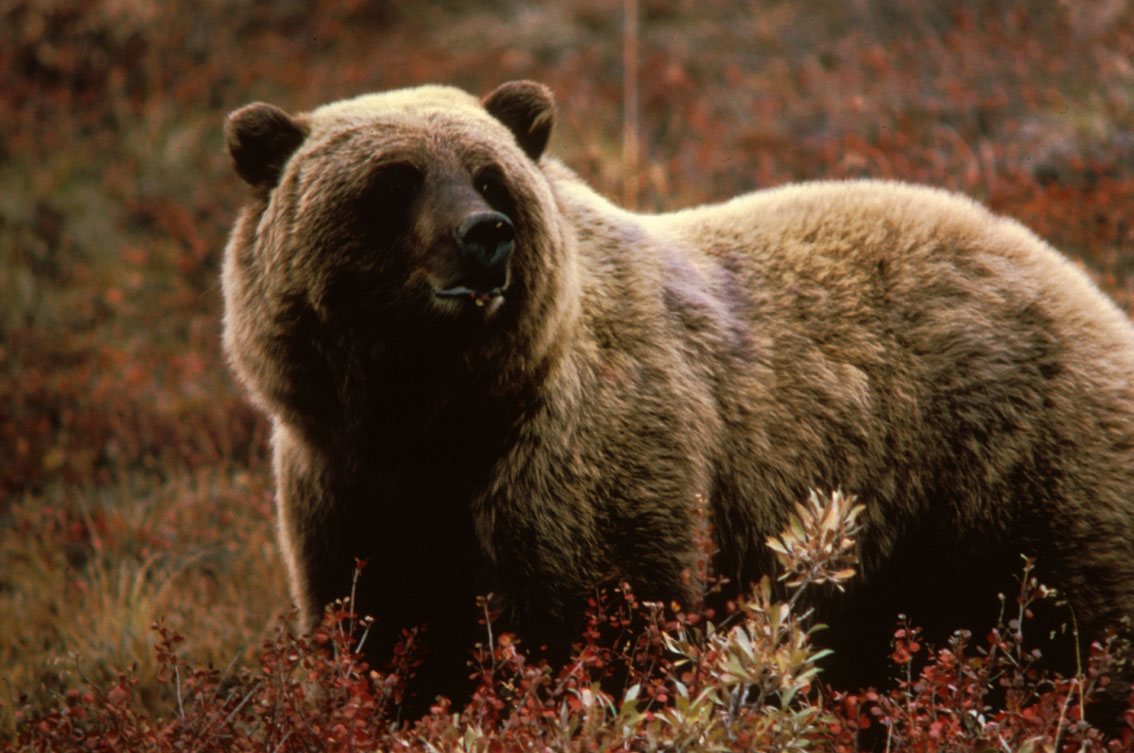
\includegraphics[width=\linewidth]{bear.jpg} % Figure image
	\caption{A majestic grizzly bear} % Figure caption
	\label{bear} % Label for referencing with \ref{bear}
\end{figure}

In hac habitasse platea dictumst. Vivamus eu finibus leo. Donec malesuada dui non sagittis auctor. Aenean condimentum eros metus. Nunc tempus id velit ut tempus. Quisque fermentum, nisl sit amet consectetur ornare, nunc leo luctus leo, vitae mattis odio augue id libero. Mauris quis lectus at ante scelerisque sollicitudin in eu nisi. Nulla elit lacus, ultricies eu erat congue, venenatis semper turpis. Ut nec venenatis velit. Mauris lacinia diam diam, ac egestas neque sodales sed. Curabitur eu diam nulla. Duis nec turpis finibus, commodo diam sed, bibendum erat. Nunc in velit ullamcorper, posuere libero a, mollis mauris. Nulla vehicula quam id tortor ornare blandit. Aenean maximus tempor orci ultrices placerat. Aenean condimentum magna vulputate erat mattis feugiat.

Quisque lacinia, purus id mattis gravida, sem enim fringilla erat, non dapibus est tellus pellentesque velit. Vivamus pretium sem quis leo placerat, at dignissim ex iaculis. Donec neque tortor, pharetra quis vestibulum id, tempus scelerisque mi. Cras in mattis est. Integer nec lorem rutrum, semper ligula bibendum, iaculis neque. Sed in nunc placerat, viverra dui in, fringilla sem. Sed quis rutrum magna, vitae pellentesque eros.

% Praesent maximus mauris vitae nisl pulvinar, at tristique tortor aliquam. Etiam sit amet nunc in nulla vulputate sollicitudin. Aliquam erat volutpat. Praesent pharetra gravida cursus. Quisque vulputate lacus nunc. Integer orci ex, porttitor quis sapien id, eleifend gravida mi. Etiam efficitur justo eget nulla congue mattis. Duis commodo vel arcu a pretium. Aenean eleifend viverra nisl, nec ornare lacus rutrum in.

% Vivamus pulvinar ac eros eu pellentesque. Duis nibh felis, sagittis sed lacus at, sagittis mattis nisi. Fusce ante dui, tincidunt in scelerisque ut, sagittis at magna. Fusce tincidunt felis et odio tincidunt imperdiet. Cras ut facilisis nisl. Aliquam vitae consequat metus, eget gravida augue. In imperdiet justo quis nulla venenatis accumsan. Aliquam aliquet consectetur tortor, at sollicitudin sapien porta sed. Donec efficitur mauris id rhoncus volutpat. Vestibulum ante ipsum primis in faucibus orci luctus et ultrices posuere cubilia Curae; Sed bibendum purus dapibus tincidunt euismod. Nullam malesuada ultrices lacus, ut tincidunt dolor. Etiam imperdiet quam eget elit tincidunt scelerisque. Curabitur ut ullamcorper dui. Cras gravida porta leo, ut lobortis nisl venenatis pulvinar. Proin non semper nulla.

% Praesent pretium nisl purus, id mollis nibh efficitur sed. Sed sit amet urna leo. Nulla sed imperdiet sem. Donec ut diam tristique, faucibus ligula vel, varius est. In ipsum ligula, elementum vitae velit ac, viverra tincidunt enim. Phasellus gravida diam id nisl interdum maximus. Ut semper, tortor vitae congue pharetra, justo odio commodo urna, vel tempus libero ex et risus. Vivamus commodo felis non venenatis rutrum. Sed pulvinar scelerisque augue in porta. Sed maximus libero nec tellus malesuada elementum. Proin non augue posuere, pellentesque felis viverra, varius urna. Lorem ipsum dolor sit amet, consectetur adipiscing elit. Donec dignissim urna eget diam dictum, eget facilisis libero pulvinar.

% Aliquam ex tellus, hendrerit sed odio sit amet, facilisis elementum enim. Suspendisse potenti. Integer molestie ac augue sit amet fermentum. Vivamus ultrices ante nulla, vitae venenatis ipsum ullamcorper sed. Phasellus gravida felis sapien, ac porta purus pharetra quis. Sed eget augue tellus. Nam vitae hendrerit arcu, id iaculis ipsum. Pellentesque sed magna tortor.

% In ac tempus diam. Sed nec lobortis massa, suscipit accumsan justo. Quisque porttitor, ligula a semper euismod, urna diam dictum sem, sed maximus risus purus sit amet felis. Fusce elementum maximus nisi a mattis. Nulla vitae elit erat. Integer sit amet commodo risus, eget elementum nulla. Donec ultricies erat sit amet sem commodo iaculis. Donec euismod volutpat lacus, ut tempor est lacinia a. Vivamus auctor condimentum tincidunt. Praesent sed finibus urna. Sed pellentesque blandit magna et rhoncus.

% Integer vel turpis nec tellus sodales malesuada a vel odio. Fusce et lectus eu nibh rhoncus tempus vel nec elit. Suspendisse commodo orci velit, lacinia dictum odio accumsan et. Vivamus libero dui, elementum vel nibh non, fermentum venenatis risus. Aliquam sed sapien ac orci sodales tempus a eget dui. Morbi non dictum tortor, quis tincidunt nibh. Proin ut tincidunt odio.

% Pellentesque ac nisi dolor. Pellentesque maximus est arcu, eu scelerisque est rutrum vitae. Mauris ullamcorper vulputate vehicula. Praesent fermentum leo ac velit accumsan consectetur. Aliquam eleifend ex eros, ut lacinia tellus volutpat non. Pellentesque sit amet cursus diam. Maecenas elementum mattis est, in tincidunt ex pretium ac. Integer ultrices nunc rutrum, pretium sapien vitae, lobortis velit.

%----------------------------------------------------------------------------------------
%	BIBLIOGRAPHY
%----------------------------------------------------------------------------------------

\printbibliography[title={Bibliography}] % Print the bibliography, section title in curly brackets

%----------------------------------------------------------------------------------------
\end{multicols}
\end{document}
